% Options for packages loaded elsewhere
\PassOptionsToPackage{unicode}{hyperref}
\PassOptionsToPackage{hyphens}{url}
%
\documentclass[
  man,
  floatsintext]{apa7}
\usepackage{amsmath,amssymb}
\usepackage{iftex}
\ifPDFTeX
  \usepackage[T1]{fontenc}
  \usepackage[utf8]{inputenc}
  \usepackage{textcomp} % provide euro and other symbols
\else % if luatex or xetex
  \usepackage{unicode-math} % this also loads fontspec
  \defaultfontfeatures{Scale=MatchLowercase}
  \defaultfontfeatures[\rmfamily]{Ligatures=TeX,Scale=1}
\fi
\usepackage{lmodern}
\ifPDFTeX\else
  % xetex/luatex font selection
\fi
% Use upquote if available, for straight quotes in verbatim environments
\IfFileExists{upquote.sty}{\usepackage{upquote}}{}
\IfFileExists{microtype.sty}{% use microtype if available
  \usepackage[]{microtype}
  \UseMicrotypeSet[protrusion]{basicmath} % disable protrusion for tt fonts
}{}
\makeatletter
\@ifundefined{KOMAClassName}{% if non-KOMA class
  \IfFileExists{parskip.sty}{%
    \usepackage{parskip}
  }{% else
    \setlength{\parindent}{0pt}
    \setlength{\parskip}{6pt plus 2pt minus 1pt}}
}{% if KOMA class
  \KOMAoptions{parskip=half}}
\makeatother
\usepackage{xcolor}
\usepackage{longtable,booktabs,array}
\usepackage{calc} % for calculating minipage widths
% Correct order of tables after \paragraph or \subparagraph
\usepackage{etoolbox}
\makeatletter
\patchcmd\longtable{\par}{\if@noskipsec\mbox{}\fi\par}{}{}
\makeatother
% Allow footnotes in longtable head/foot
\IfFileExists{footnotehyper.sty}{\usepackage{footnotehyper}}{\usepackage{footnote}}
\makesavenoteenv{longtable}
\usepackage{graphicx}
\makeatletter
\newsavebox\pandoc@box
\newcommand*\pandocbounded[1]{% scales image to fit in text height/width
  \sbox\pandoc@box{#1}%
  \Gscale@div\@tempa{\textheight}{\dimexpr\ht\pandoc@box+\dp\pandoc@box\relax}%
  \Gscale@div\@tempb{\linewidth}{\wd\pandoc@box}%
  \ifdim\@tempb\p@<\@tempa\p@\let\@tempa\@tempb\fi% select the smaller of both
  \ifdim\@tempa\p@<\p@\scalebox{\@tempa}{\usebox\pandoc@box}%
  \else\usebox{\pandoc@box}%
  \fi%
}
% Set default figure placement to htbp
\def\fps@figure{htbp}
\makeatother
\setlength{\emergencystretch}{3em} % prevent overfull lines
\providecommand{\tightlist}{%
  \setlength{\itemsep}{0pt}\setlength{\parskip}{0pt}}
\setcounter{secnumdepth}{-\maxdimen} % remove section numbering
% definitions for citeproc citations
\NewDocumentCommand\citeproctext{}{}
\NewDocumentCommand\citeproc{mm}{%
  \begingroup\def\citeproctext{#2}\cite{#1}\endgroup}
\makeatletter
 % allow citations to break across lines
 \let\@cite@ofmt\@firstofone
 % avoid brackets around text for \cite:
 \def\@biblabel#1{}
 \def\@cite#1#2{{#1\if@tempswa , #2\fi}}
\makeatother
\newlength{\cslhangindent}
\setlength{\cslhangindent}{1.5em}
\newlength{\csllabelwidth}
\setlength{\csllabelwidth}{3em}
\newenvironment{CSLReferences}[2] % #1 hanging-indent, #2 entry-spacing
 {\begin{list}{}{%
  \setlength{\itemindent}{0pt}
  \setlength{\leftmargin}{0pt}
  \setlength{\parsep}{0pt}
  % turn on hanging indent if param 1 is 1
  \ifodd #1
   \setlength{\leftmargin}{\cslhangindent}
   \setlength{\itemindent}{-1\cslhangindent}
  \fi
  % set entry spacing
  \setlength{\itemsep}{#2\baselineskip}}}
 {\end{list}}
\usepackage{calc}
\newcommand{\CSLBlock}[1]{\hfill\break\parbox[t]{\linewidth}{\strut\ignorespaces#1\strut}}
\newcommand{\CSLLeftMargin}[1]{\parbox[t]{\csllabelwidth}{\strut#1\strut}}
\newcommand{\CSLRightInline}[1]{\parbox[t]{\linewidth - \csllabelwidth}{\strut#1\strut}}
\newcommand{\CSLIndent}[1]{\hspace{\cslhangindent}#1}
\ifLuaTeX
\usepackage[bidi=basic]{babel}
\else
\usepackage[bidi=default]{babel}
\fi
% get rid of language-specific shorthands (see #6817):
\let\LanguageShortHands\languageshorthands
\def\languageshorthands#1{}
% preamble.tex 

\usepackage{csquotes}
\usepackage{amsmath}
\usepackage{amssymb}
\usepackage{graphicx}
\usepackage{subcaption}
\usepackage{caption}
\usepackage{geometry}
\usepackage{float}
\usepackage{rotating}


\captionsetup{justification=raggedright,singlelinecheck=false}

\shorttitle{SEMI-COMPLETE BY DESIGN}
\affiliation{$^{1}$Goethe University Frankfurt\\ $^{2}$Max Planck Institute for Human Development{,} Berlin{,} Germany\\ $^{3}$MSB Medical School Berlin{,} Berlin{,} Germany\\ $^{4}$Max Planck UCL Centre for Computational Psychiatry and Ageing Research{,} Berlin{,} Germany}
\abstract{Abstract text goes here.}

\keywords{Measurement invariance, moderated nonlinear factor analysis, structural equation model trees, continuous moderators, Monte Carlo simulation}
\usepackage{placeins}
\usepackage{float}
\usepackage{threeparttable}
\setlength{\textfloatsep}{6pt}
\setlength{\floatsep}{6pt}
\setlength{\intextsep}{6pt}
\raggedbottom
\usepackage{bookmark}
\IfFileExists{xurl.sty}{\usepackage{xurl}}{} % add URL line breaks if available
\urlstyle{same}
\hypersetup{
  pdftitle={Testing Measurement Invariance with Continuous Covariates: Comparing Moderated Nonlinear Factor Analysis and Structural Equation Model Trees},
  pdfauthor={Leonie Hagitte\^{}\{1,2,3\}, Andreas M. Brandmaier\^{}\{2,3,4\}},
  pdflang={american},
  pdfkeywords={Measurement invariance, Moderated nonlinear factor
analysis, Structural equation model trees, Continuous moderators, Monte
Carlo simulation},
  hidelinks,
  pdfcreator={LaTeX via pandoc}}

\title{Testing Measurement Invariance with Continuous Covariates:
Comparing Moderated Nonlinear Factor Analysis and Structural Equation
Model Trees}
\author{Leonie Hagitte\(^{1,2,3}\), Andreas M. Brandmaier\(^{2,3,4}\)}
\date{2026-09-16}

\begin{document}
\maketitle

Meaningful comparisons between individuals or groups of individuals
depend on the assumption that psychological constructs are measured in
the same way across various contexts. Unlike weight or height of a
person, latent constructs such as intelligence, attitudes, or
personality traits are not directly observable. Instead, researchers
infer them from responses to observed indicators using measurement
models. Ensuring that these measurements operate equivalently is
therefore a prerequisite for valid scientific conclusions.

When a measure fails to represent the intended construct or functions
differently across individuals, groups, or contexts, even highly
rigorous analyses may produce misleading conclusions (Flake and Fried
2020; Flake, Pek, and Hehman 2017). Thus, a central aspect of
measurement quality is \emph{measurement invariance} (MI), which refers
to the assumption that a measurement model operates equivalently across
individuals, groups, contexts, or measurement occasions.

When MI holds, the relationship between a latent construct and its
observed indicators remains stable across the conditions being compared
(Meredith 1993). Thus, assuming MI is essential whenever researchers
seek to compare latent means, variances, covariances, or structural
relations, making MI a fundamental prerequisite for correlational,
experimental, and longitudinal research designs (Putnick and Bornstein
2016; Little 1997).\\
Conversely, violations of MI indicate that observed differences may
reflect not only substantive differences in the underlying construct but
also systematic differences in item functioning or measurement precision
(Cheung and Rensvold 2002; Meredith 1993). Without establishing MI, it
is therefore impossible to determine whether observed differences
reflect true differences in the latent construct or artifacts of the
measurement process. Consequently, MI is not only a methodological
requirement but also a prerequisite for valid theoretical
interpretation.

Conventional approaches to MI typically represent heterogeneity in
measurement parameters through predefined groups or discrete conditions.
This representation becomes restrictive when candidate sources of
measurement heterogeneity are continuous, such as age or other
individual characteristics, particularly when the functional
relationships between these covariates and measurement parameters are
unknown. In these settings, discretizing continuous covariates may
obscure the form and location of measurement non-invariance, whereas
imposing a prespecified functional relationship risks misspecifying the
underlying heterogeneity. Thus, a central methodological problem is how
to represent and detect heterogeneity in measurement parameters across
continuous covariates without requiring either predefined groups or a
known functional form.

\subsection{Classical Measurement Invariance
Testing}\label{classical-measurement-invariance-testing}

Structural equation models (SEMs) are widely used to define latent
constructs and their relations to observed indicators (Kline 2023;
Kenneth A. Bollen and Noble 2011; Tarka 2018). Within SEMs, measurement
models specify the relationships between latent factors and their
manifest indicators. By separating construct-related variance from
measurement error, latent variable models provide a principled basis for
evaluating measurement quality (K. A. Bollen 1989).

Classical approaches to MI testing are fundamentally confirmatory in
nature. Researchers begin by specifying a measurement model, typically
in the form of a confirmatory factor analysis (CFA), that reflects
substantive hypotheses about the construct under investigation. A
categorical grouping variable is then used to partition the sample into
two or more groups, across which measurement parameters are constrained
and compared. This most widely used approach for evaluating MI is
usually referred to as multiple-group confirmatory factor analysis
(MGCFA) (e.g. Cheung and Rensvold 2002; Putnick and Bornstein 2016).\\
In MGCFA, MI is typically assessed through a sequence of nested model
comparisons in which increasingly restrictive equality constraints are
imposed on the model parameters. Equality of the models structure in
both groups is called \emph{configural invariance}, and can be
understood as both groups sharing the same factor structure (i.e., same
number of latent factors and same pattern of loadings between factors
and items). Equality of factor loadings former is referred to as
\emph{metric invariance}, if metric invariance is present it indicates
that all factor loading parameters are equal across groups. Specifically,
this suggests that the items of a given scale and their underlying
constructs relate to each other with the same strengths in both groups.
\emph{Scalar invariance} further constrains item intercepts to equality
across groups. Establishing scalar invariance is required for meaningful
comparisons of latent means because it indicates that the measurement
scale has the same unit and origin across groups (Little 1997).
\emph{Residual} or \emph{strict invariance} assumes, additionally to the
constraints above, that variables residuals are equal across the groups.
If residual variance holds, the items of the scale are measuring the
latent constructs with the same measurement error. This implies that it
can indeed be known whether differences measured by the items of the
tested scale between the groups are due to group differences in the
proposed factors or due to measurement errors (Cheung and Rensvold 2002;
Widaman and Reise 1997).

The appropriate level of invariance required depends on the substantive
inference of interest. For example, metric invariance is generally
required when comparing latent means across groups, whereas less
restrictive forms of invariance may be sufficient for research questions
about correlations (Putnick and Bornstein 2016).

In MGCFA, MI testing depends on the specified measurement model and
grouping variable. Accordingly, measurement noninvariance (MNI) can only
be detected with respect to the grouping variables included in the
analysis. This framework is well suited to settings in which theory
implies meaningful discrete distinctions, such as treatment conditions,
demographic categories, or measurement occasions. However, many
characteristics that may affect measurement functioning vary
continuously across individuals. Converting such characteristics into
predefined groups may require arbitrary cutoffs and obscure relevant
variation in measurement parameters.

Additionally, categorization may obscure how measurement parameters vary
along the underlying continuous characteristic. Methods for representing
heterogeneity in measurement parameters across continuous covariates are
therefore needed when neither discrete groups nor the functional form of
parameter variation can be specified a priori.

\subsection{Moderated Nonlinear Factor
Analysis}\label{moderated-nonlinear-factor-analysis}

Moderated nonlinear factor analysis (MNLFA) meets this requirement by
modeling factor loadings, intercepts, and other measurement parameters
as functions of observed covariates, including continuous
characteristics (Bauer and Hussong 2009; Bauer 2017). In this way, MNLFA
extends conventional group-based invariance testing by representing
measurement heterogeneity without imposing arbitrary group boundaries.
MNI is conceptualized as moderation of the measurement model itself by
variables exogenous to the model. If measurement parameters differ as a
function of these moderator variables, the measurement model no longer
operates equivalently across individuals and therefore violates MI
(Bauer 2017; Kolbe et al. 2024).

Hence, whether MI is present depends on which parameters are moderated
by the exogenous variables. The exogenous variables may moderate any
subset of the parameters in the measurement model and structural model.
Specifically, the means, variances, and covariance of latent factors, as
well as the item intercepts, factor loadings, and residual variances of
any manifest indicator, may vary systematically across individuals as
deterministic functions of the exogenous variable (Bauer and Hussong
2009; Bauer 2017). If moderation is limited to the latent-factor
parameters, that is, the means, variances, and covariance, the model
remains consistent with MI. In contrast, moderation of item-level
parameters, including intercepts, loadings, or residual variances,
constitutes MNI (Bauer 2017; Kolbe et al. 2024). Accordingly, a
moderation function must be specified for each parameter that is allowed
to vary as a function of the exogenous variable. Because of this
conceptualization,this method allows researchers to model gradual,
nonlinear, and individual-specific forms of MNI that are difficult to
represent within traditional multiple-group approaches (Bauer and
Hussong 2009; Kolbe et al. 2024).

This increased flexibility comes at the cost of greater specification
requirements. Like MGCFA, MNLFA constitutes a confirmatory approach to
the assessment of MI (Bauer 2017). In practice, at least three sets of
decisions are required. First, the measurement model must be specified,
including the latent structure and the relationships between latent and
observed variables. Second, one or more moderator variables must be
selected to represent potential sources of heterogeneity in the
measurement process. Third, moderation functions must be specified for
all parameters that are allowed to vary as a function of the moderator.
This includes determining which parameters are moderated as well as
specifying the functional form of each moderation effect (e.g., linear,
quadratic, or another parametric form). Consequently, the detection of
MNI depends not only on the choice of moderator variables but also on
the assumptions made about how these moderators influence the model
parameters (Bauer and Hussong 2009; Bauer 2017).

This specification becomes challenging when there is limited prior
knowledge about which candidate covariates are associated with
measurement parameters, which parameters exhibit heterogeneity, or what
functional forms characterize these relationships. Such settings
motivate methods that can explore parameter heterogeneity without
requiring these moderation relationships to be fully specified a priori.

\subsection{Structural Equation Model
Trees}\label{structural-equation-model-trees}

Structural Equation Model trees (SEM trees) were originally introduced
by Brandmaier et al.~(2013) as a method for identifying important
covariates and their interactions within SEMs to explain heterogeneity,
e.g., by identifying moderators of model parameters in a SEM. Subsequent
developments further refined the methodology and expanded its
applicability (Arnold et al., 2021; Brandmaier et al., 2016).
finch2017structural Notably, SEM Trees were not developed as a dedicated
methods to investigate measurement invariance but as a generic strategy
for explaining heterogeneity. Because violations of MI manifest as
systematic heterogeneity in parameters of the measurement model, SEM
trees are by design well suited for detecting such effects. Even though
SEM Trees have received relatively little attention as tools for
detecting MNI in general, some researchers have already used SEM Trees
as a successful heuristic to investigate measurement invariance Sajobi
et al. (2026).

SEM trees merge two paradigms: SEMs and decision trees. Decision trees
describe recursive partitions of the covariate space, whereby the sample
is repeatedly split according to covariate values into progressively
more homogeneous subsets, in order to maximize differences in a given
outcome variable. SEM Trees combine the hierarchical structure of
decision trees with SEMs, so that they describe heterogeneity in data
with respect to a specified SEM as targeted outcome structure. Unlike
many other tree-based methods, SEM Trees can be applied to models that
include latent variables.

In contrast to MGCFA and MNLFA, SEM trees represent a rather exploratory
approach to the assessment of MI. Similar to these methods, SEM trees
require the researcher to specify a measurement model a priori. Beyond
this, however, the researcher only needs to provide a set of candidate
variables that may account for heterogeneity in the data. These
variables may be numerous and can be either categorical or continuous.\\
Similar to MGCFA, researchers first specify a measurement model and
identify variables that may account for heterogeneity. The crucial
difference is that MGCFA requires the researcher to select a specific
categorical grouping variable, whereas SEM trees can evaluate a large
set of candidate variables simultaneously and determine which, if any,
are associated with violations of MI. Moreover, SEM trees can
accommodate heterogeneity generated by nonlinear forms of moderation
without requiring the functional form to be specified parametrically, by
representing such heterogeneity through recursive partitioning.

Hence, SEM trees combine a theory-driven measurement model with a
data-driven search for heterogeneity. This makes them especially
valuable when researchers have a well-established measurement model but
little prior knowledge about where MNI may arise or what form it may
take. Because the decision structure closely resembles familiar MGCFA
practice, SEM trees represent a comparatively accessible extension of
conventional MI analysis.

This highlights, that SEM trees can offer substantially greater
flexibility by accommodating multiple candidate moderators, continuous
and categorical partitioning variables, and potentially nonlinear
functional forms to explain heterogeneity, given the sample size is
large enough to detect such effects. Although explicit specification of
moderators and moderation functions remains advantageous when strong
theoretical expectations are available, SEM trees could provide a
complementary strategy for situations in which the sources or functional
forms of heterogeneity are uncertain.

\subsection{Present Study}\label{present-study}

MGCFA, MNLFA, and SEM trees differ in how they represent heterogeneity
in measurement parameters. MGCFA captures heterogeneity as differences
between predefined groups. When heterogeneity is associated with a
continuous covariate \((z)\), the problem can instead be framed as
modeling a measurement parameter \((\theta)\) as a function of that
covariate, \((\theta(z))\), as in MNLFA. MNLFA represents this
relationship using parametrically specified moderation functions,
whereas SEM trees use data-driven recursive partitions of the covariate
space. The methods therefore differ in how they represent the
relationship between covariates and measurement parameters.

The present simulation study examines the consequences of these
different representations for detecting MNI. Specifically, we compare
MNLFA and SEM trees performance in detecting MNI, when the true
parameter--covariate relationship is linear, quadratic, or sigmoidal,
while additionally varying the magnitude of parameter heterogeneity and
sample size.

The comparison addresses three aspects of performance. First, we examine
whether each method detects the presence of MNI. Second, we evaluate how
detection depends on the functional form of \(\theta(z)\), thereby
assessing the consequences of representing parameter heterogeneity
parametrically or through recursive partitions. Third, because the
simulation separately introduces heterogeneity in factor loadings and
item intercepts, we examine whether the methods correctly identify the
level at which MNI occurs, corresponding to metric and scalar MNI for
continuous indicators.

We expect SEM trees to perform particularly well in conditions
characterized by nonlinear moderation, especially sigmoidal
relationships, whereas their relative advantage should diminish in
purely linear settings. In contrast, MNLFA is expected to perform best
when the functional form of moderation is correctly specified,
particularly in linear conditions, but to be more sensitive to
misspecification of the underlying moderation function. For both
methods, stronger moderation effects are expected to increase the
detectability of measurement non-invariance.

Related tree-based approaches have recently been developed specifically
for investigating MNI across multiple covariates within the broader
SEM-tree framework. Sterner and Goretzko (2023) introduced exploratory
factor analysis (EFA) trees, and Goretzko, Howard, and Sterner (2026)
subsequently extended this work to CFA trees. Like SEM trees more
generally, EFA and CFA trees use model-based recursive partitioning and
score-based structural-change tests to identify parameter instability
across candidate covariates. EFA trees embed an exploratory factor model
within this framework, whereas CFA trees retain a prespecified
confirmatory measurement structure and can be configured to investigate
particular classes of measurement parameters, including item intercepts
in analyses of scalar MNI.

The procedure examined in the present study is a CFA-based application
of the generic SEM-tree framework. Metric and scalar MNI are
investigated using separate score-based instability tests focused on
factor loadings and item intercepts, respectively. This
parameter-focused implementation differs in its constraint strategy from
the intercept-focused CFA-tree procedure described by Goretzko, Howard,
and Sterner (2026), in which nonfocal model parameters can be fixed
while intercepts are evaluated for instability. Rather than proposing a
distinct tree-based MI method, the present study therefore evaluates the
performance of a particular parameter-focused specification of SEM trees
and compares it with the parametric moderation approach of MNLFA.

In addition to the simulation study, we compare the results of both
approaches for assessing measurement invariance with metric predictors
data using empirical data from the ninth wave of the Survey of Health,
Ageing and Retirement in Europe (SHARE-ERIC 2024). As primary outcome,
we model quality of life assessed by the CASP-12 (Borrat-Besson, Ryser,
and Goncalves 2015; Wiggins et al. 2008). The illustration is motivated
by the study from Bonneville-Roussy, Khoriaty, and Laberge (2024), who
examined longitudinal and cross-sectional MI of the CASP-12 across age,
gender, and cultural regions using group-based comparisons. Age is a
particularly useful case for comparison: conventional MGCFA, which
requires discretizing continous age into age groups, whereas the
approaches considered here can incorporate age as a continuous
covariate, avoiding potentially arbitrary categorization.

We close with an integrative discussion of the simulation and empirical
results and give some practical recommendations to researcher as to when
each approach, that is a conventional MGCFA, MLNFA, or SEM Trees may be
best suitable to examine measurement invariance in latent variable
models.

\section{Method}\label{method}

\subsection{Simulation}\label{simulation}

\subsection{Data-generating mechanism}\label{data-generating-mechanism}

Data were generated from a single-factor CFA model measured by four
continuous indicators. Baseline factor loadings were fixed to
\(\lambda = 0.70\), baseline intercepts were fixed to one, and the
latent factor variance was fixed to one.

Residual variances were fixed such that indicator reliability equaled
\(\rho = .75.\) at the baseline factor loading of \(\lambda=.70\).
Because residual variances were held constant while loadings varied
under loading moderation, conditional indicator reliability varied
accordingly in conditions with metric noninvariance. MNI was introduced
by allowing selected factor loadings and/or item intercepts to depend on
the moderator.

Nine population models were investigated.

\begin{table}[ht]
\centering
\begin{threeparttable}
\caption{Overview of the moderation models.}

\begin{tabular}{lll}
\toprule
Model & Loading moderation & Intercept moderation\\
\midrule
L0I0 & none & none\\
LAI0 & all items & none\\
L0IA & none & all items\\
LAIA & all items & all items\\
L2I0 & items 1--2 & none\\
\addlinespace
L0I2 & none & items 1--2\\
L2I2 & items 1--2 & items 1--2\\
\bottomrule
\end{tabular}
\begin{tablenotes}[flushleft]
\footnotesize
\item \textit{Note.} L = loading; I = intercept; 0 = no moderation; 2 = moderation of items 1--2; A = moderation of all items.
\end{tablenotes}
\end{threeparttable}
\end{table}

MNI was generated by allowing selected measurement parameters to vary
continuously as deterministic functions of an observed moderator
variable. For each simulated individual, a moderator
\(M \sim \mathcal U(-1,1)\) was sampled from a continuous uniform
distribution and transformed into an effective moderator\(Z = h(M)\),
where the transformation \(h(\cdot)\) determined the functional form of
moderation. Measurement parameters were subsequently modeled as linear
functions of the transformed moderator. Consequently, any nonlinearity
in parameter variation arose exclusively through the transformation
\(h(\cdot)\).

\subsubsection{Functional forms of
moderation}\label{functional-forms-of-moderation}

Four moderator functions were considered:

\begin{enumerate}
\def\labelenumi{\arabic{enumi}.}
\tightlist
\item
  \textbf{Linear:} \[
  h(M) = M
  \]
\end{enumerate}

In this case, the effective moderator is bounded to the interval
\((-1,1)\) and rotation symmetric around zero.

\begin{enumerate}
\def\labelenumi{\arabic{enumi}.}
\setcounter{enumi}{1}
\item
  \textbf{Sigmoid:} \[
  h(M) = a + \frac{b-a}{1 + \exp\!\bigl(-k(M-c)\bigr)},
  \qquad a=-1,\; b=1,\; c=0,\; k>0.
  \] This transformation maps the input to the open interval \((-1, 1)\)
  and yields a bounded moderator, rotation symmetric around zero,
  exhibiting diminishing sensitivity at extreme values. In our
  simulation \(k\) is set to 10.
\item
  \textbf{Quadratic:} \[
  h(M) = 2M^2 - 1
  \] This transformation captures symmetric nonlinear moderation as a
  function of distance from the center while remaining bounded in
  \((-1,1)\).
\item
  \textbf{Null:} \[
  h(M) = 0
  \]
\end{enumerate}

These functions were selected to represent qualitatively different forms
of heterogeneity. The first three functions represented structured forms
of moderation, whereas the noise condition represented the absence of
systematic moderation. All moderator transformations were bounded to the
interval \((-1,1)\), implying identical maximum parameter deviations for
a given moderation coefficient, but not necessarily the same variance.
Consequently, identical values of the moderation coefficient imply
identical maximum parameter deviations but not necessarily identical
average parameter variation.

\begin{figure}

{\centering 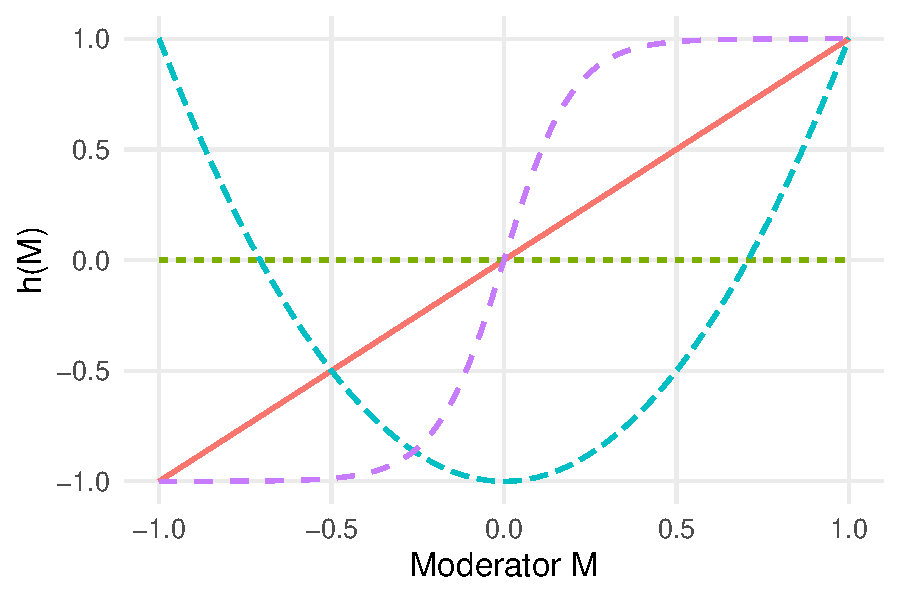
\includegraphics[width=0.75\linewidth]{semi_manuscript_files/figure-latex/my-figure-1} 

}

\caption{figure caption.}\label{fig:my-figure}
\end{figure}

\subsection{Simulation design}\label{simulation-design}

The simulation crossed data-generating conditions with analysis method.
Data-generating conditions manipulated The manipulated data-generating
factors are summarized in Table (\textbf{ref?})(tab:simulation-design).

\begin{longtable}[]{@{}
  >{\raggedright\arraybackslash}p{(\linewidth - 2\tabcolsep) * \real{0.3974}}
  >{\raggedright\arraybackslash}p{(\linewidth - 2\tabcolsep) * \real{0.6026}}@{}}
\caption{Overview of the simulation design.}\tabularnewline
\toprule\noalign{}
\begin{minipage}[b]{\linewidth}\raggedright
Factor
\end{minipage} & \begin{minipage}[b]{\linewidth}\raggedright
Levels
\end{minipage} \\
\midrule\noalign{}
\endfirsthead
\toprule\noalign{}
\begin{minipage}[b]{\linewidth}\raggedright
Factor
\end{minipage} & \begin{minipage}[b]{\linewidth}\raggedright
Levels
\end{minipage} \\
\midrule\noalign{}
\endhead
\bottomrule\noalign{}
\endlastfoot
Population model & 0, 1.1, 1.11, 1.12, 1.2, 1.21, 1.22, 1.3, 1.32 \\
Functional form of moderation & Linear, quadratic, sigmoid, null/no
moderation \\
Loading moderation magnitude & \(\delta_\lambda \in \{0.20, 0.30\}\) \\
Intercept moderation magnitude & \(\delta_\nu \in \{0.50, 1.00\}\) \\
Sample size & \(N \in \{300, 500, 700, 1000\}\) \\
Indicator reliability & \(\rho = .75\) \\
Baseline factor loading & \(\lambda = .70\) \\
Baseline item intercept & \(\nu = 1\) \\
Analysis method & Linear MNLFA, quadratic MNLFA, SEM tree \\
\end{longtable}

\subsubsection{Primary and exploratory simulation
conditions}\label{primary-and-exploratory-simulation-conditions}

The combination of the nine population models, four functional forms,
two loading-moderation magnitudes, two intercept-moderation magnitudes,
and four sample sizes resulted in 576 primary data-generating design
cells. Each condition was evaluated using linear MNLFA, quadratic MNLFA,
and SEM trees across 100 replications, yielding 172,800 primary
analyses.

Inspection of the primary results indicated that several conditions
yielded near-ceiling detection rates, limiting differentiation between
methods at the preregistered effect sizes. Exploratory sensitivity
analyses therefore additionally examined smaller moderation effects
\((\delta_\lambda=.10, \delta_\nu=.25)\); these conditions were analyzed
separately from the primary conditions.

In the primary method comparison, the relevant data-generating moderator
or moderators were supplied to the SEM trees as candidate partitioning
variables. Thus, the comparison focused on how the methods represent
moderator-related parameter heterogeneity. Candidate-variable selection
was examined separately in a robustness analysis.

\subsection{Analysis Models}\label{analysis-models}

The simulated population conditions were evaluated using two
parametrically specified MNLFA analyses, linear MNLFA and quadratic
MNLFA, as well as score-based SEM trees. All analyses were based on a
single-factor measurement model with four continuous indicators
\(x_1,\ldots,x_4\) and one latent factor \(\eta\). The MNLFA analyses
evaluated metric and scalar MNI through nested likelihood-ratio tests,
whereas the SEM-tree analyses used separate score-based
parameter-instability tests focused on factor loadings and item
intercepts.

\subsubsection{MNLFA}\label{mnlfa}

MNLFA models were estimated in \texttt{OpenMx} using raw-data maximum
likelihood. The latent-factor mean and variance were fixed to 0 and 1,
respectively, for identification. Baseline item intercepts, factor
loadings, and residual variances were freely estimated.

Let \(M_1\) and \(M_2\) denote the raw moderator variables. In the
data-generating model, the effective moderators were defined as
\(Z_k^{(d)}=h(M_k)\), where \(h(\cdot)\) denotes the data-generating
transformation. For the fitted MNLFA, we analogously define the
analysis-scale effective moderators as\(Z_k^{(a)}=g(M_k)\), where
\(g(\cdot)\) denotes the transformation assumed in the analytical model.
For conditions involving two moderators, the interaction term was
defined as \(Z_{12}^{(a)}=Z_1^{(a)}Z_2^{(a)}\). In the unrestricted
MNLFA, the intercept of item \(i\) was specified as

\[
\nu_i\left(Z_1^{(a)},Z_2^{(a)}\right)
=
\nu_{i0}
+
\beta_{\nu i1}Z_1^{(a)}
+
\beta_{\nu i2}Z_2^{(a)}
+
\beta_{\nu i12}Z_{12}^{(a)},
\] and its factor loading as

\[
\lambda_i\left(Z_1^{(a)},Z_2^{(a)}\right)
=
\lambda_{i0}
+
\beta_{\lambda i1}Z_1^{(a)}
+
\beta_{\lambda i2}Z_2^{(a)}
+
\beta_{\lambda i12}Z_{12}^{(a)}.
\]

Thus, moderator effects associated with \(Z_1^{(a)}\), \(Z_2^{(a)}\),
and their interaction \(Z_{12}^{(a)}\) were freely estimated for every
item intercept and factor loading. Residual variances were additionally
allowed to vary with \(Z_1^{(a)}\) and \(Z_2^{(a)}\) according to the
log-linear specification

\[
\theta_i\left(Z_1^{(a)},Z_2^{(a)}\right)
=
\theta_{i0}
\exp\left(
\gamma_{i1}Z_1^{(a)}
+
\gamma_{i2}Z_2^{(a)}
\right).
\]

Residual-variance moderation was included as a nuisance component of the
fitted MNLFA and was not used to define metric or scalar MNI. No
interaction term was included for residual-variance moderation. The
latent mean was fixed at zero and was not moderated, and the latent
variance was fixed at one.

Metric MNI was evaluated by comparing the unrestricted model with a
metric-invariance model in which all moderator effects on the factor
loadings were constrained to zero. Moderator effects on item intercepts
and residual variances remained freely estimated. The resulting
likelihood-ratio test therefore evaluated the joint null hypothesis that
the factor loadings did not vary as a function of the modeled
moderators. Scalar MNI was evaluated by comparing the metric-invariance
model with a scalar-invariance model in which moderator effects on item
intercepts were additionally constrained to zero. Residual-variance
moderation remained freely estimated. The scalar likelihood-ratio test
therefore evaluated the joint null hypothesis of no moderator-related
intercept variation conditional on loading moderation having been
constrained to zero. An additional omnibus comparison between the
unrestricted and scalar-invariance models tested the joint removal of
loading and intercept moderation. All likelihood-ratio tests used
\(\alpha=.05\).

The linear and quadratic MNLFA conditions differed only in the
transformation \(g(\cdot)\) applied to the raw moderators before they
entered the moderation equations. In the \emph{linear MNLFA},\(g(M)=M\),
such
that\(Z_1^{(a)}=M_1,\qquad Z_2^{(a)}=M_2,\qquad Z_{12}^{(a)}=M_1M_2\).

In the \emph{quadratic MNLFA}, \(g(M)=2M^2-1\), such that
\(Z_1^{(a)}=2M_1^2-1, \qquad Z_2^{(a)}=2M_2^2-1\), and \$
Z\_\{12\}\^{}\{(a)\} = Z\_1\textsuperscript{\{(a)\}Z\_2}\{(a)\}\$.

Thus, the quadratic MNLFA did not represent a conventional polynomial
model containing both a linear and a squared moderator term. Rather, it
used the quadratically transformed effective moderator in otherwise
identical moderation equations. Both MNLFA specifications were linear in
the supplied effective moderator \(Z^{(a)}\). The analytical functional
form was therefore correctly specified when \(g(\cdot)=h(\cdot)\) and
misspecified otherwise. Accordingly, linear MNLFA matched the linear DGM
and quadratic MNLFA matched the quadratic DGM. No sigmoid MNLFA
specification was fitted; consequently, both MNLFA specifications were
functionally misspecified under sigmoid data-generating conditions.

\subsubsection{Score-based SEM trees}\label{score-based-sem-trees}

For the SEM-tree analyses, a single-factor CFA was specified with all
four factor loadings \(\lambda_1,\ldots,\lambda_4\), all four item
intercepts \(\nu_1,\ldots,\nu_4\), and all four residual variances
freely estimated. The latent-factor mean and variance were fixed at 0
and 1, respectively. This CFA served as the base model for recursive
partitioning.

Separate SEM trees were estimated for loading-related and
intercept-related parameter instability. In the \emph{metric tree}, the
four factor-loading parameters \(\lambda_1,\ldots,\lambda_4\) were
specified as \texttt{focus.parameters} in the score-based instability
tests. Candidate splits were therefore evaluated with respect to
instability in the loading parameters. In the \emph{scalar tree}, the
four item-intercept parameters \(\nu_1,\ldots,\nu_4\) were instead
specified as \texttt{focus.parameters}, such that the instability test
targeted heterogeneity in the intercept parameters.

Importantly, \texttt{focus.parameters} determined which parameter scores
entered the instability test; non-focused free parameters were not
globally fixed. Thus, item intercepts and residual variances remained
free parameters of the CFA underlying the loading-focused tree, whereas
factor loadings and residual variances remained free parameters of the
CFA underlying the intercept-focused tree. The metric and scalar SEM
trees therefore constituted separate parameter-focused instability
analyses rather than a sequence of CFA models in which increasingly
restrictive equality constraints were imposed on the complete
measurement model. This implementation detail is particularly relevant
for interpreting cross-level rejection, because instability detected by
a loading-focused or intercept-focused test need not imply that
heterogeneity is confined exclusively to the corresponding parameter
class.

Recursive partitioning used score-based parameter-instability tests with
\(\alpha=.05\), Bonferroni adjustment for multiple testing, a maximum
tree depth of three, and a minimum node size of 50.

In the primary comparison, SEM trees were supplied with the relevant raw
data-generating moderator \(M_1\), or moderators \(M_1\) and \(M_2\), as
candidate partitioning variables. Unlike MNLFA, the SEM-tree analyses
were therefore not supplied with the effective transformed moderators
\(Z^{(d)}=h(M)\). Under quadratic and sigmoid data-generating
conditions, the tree instead had to represent the resulting parameter
heterogeneity through recursive partitions of the original moderator
space \(M\).

Candidate-variable selection was examined separately in a robustness
analysis. In this condition, the true raw moderator \(M_1\) was
supplemented with ten independent irrelevant predictors, each generated
independently from a uniform distribution on \((-1,1)\). The robustness
analysis was restricted to the all-item metric-MNI condition with linear
moderation, \(N=500\), \(\delta_\lambda=.20\), and \(\delta_\nu=.50\).
It therefore evaluated whether the SEM tree could select the informative
moderator when irrelevant candidate partitioning variables were also
available.

\subsection{Evaluation criteria}\label{evaluation-criteria}

Performance was evaluated separately for metric and scalar MNI. For
MNLFA, metric and scalar MNI were assessed using sequential
likelihood-ratio tests comparing nested moderation models. For SEM
trees, MNI was assessed using score-based global parameter-instability
tests on the respective focus parameters (factor loadings or intercepts)
with Bonferroni-adjusted significance tests.

For each population model and simulation condition, the following
performance measures were computed:

\textbf{Statistical power:} The proportion of simulation replications in
which the method rejected the null hypothesis of MI at the corresponding
level when the respective form of MNI was present in the data-generating
model.

\textbf{Complete-null rejection:} The proportion of simulation
replications in which the method rejected the null hypothesis of MI at
the corresponding level under complete MI, when neither loading nor
intercept MNI was present.

\textbf{Level-specific rejection:} The proportion of simulation
replications in which the method rejected the null hypothesis of MI at
the corresponding level when that form of MNI was absent, but MNI could
be present at another level. For example, metric rejection under
scalar-only MNI was considered level-specific rejection rather than
rejection under complete MI.

In addition, a \textbf{sequential classification} was derived using a
metric-first decision rule, following traditional approaches to MI
testing. If the metric test rejected, the replication was classified as
metric MNI; if the metric test did not reject but the scalar test
rejected, it was classified as scalar MNI; if neither test rejected,
invariance was retained. In the primary comparison, SEM trees were
supplied only with the true moderator variables. Consequently,
statistical power and rejection rates reflect the ability to detect MNI
independent of moderator selection.

In the robustness analysis a simulation replication was considered
successful only if the SEM tree both rejected the null hypothesis of
parameter stability and selected the true moderator as a splitting
variable. This criterion therefore jointly evaluated the ability of SEM
trees to detect MNI and to distinguish the informative moderator from
irrelevant candidate predictors.

\subsection{Replications}\label{replications}

Each data-generating design cell was replicated 100 times. The three
analysis methods were evaluated in separate method-specific simulation
runs. Method-specific replications used independently seeded datasets,
and performance was therefore compared at the simulation-condition level
rather than through paired replication-level contrasts. An additional
100 SEM-tree analyses were conducted for the noisy-predictor robustness
condition.

\subsection{Empirical Example}\label{empirical-example}

We analyzed the CASP-12 using data from Wave 9 of the Survey of Health,
Ageing and Retirement in Europe (SHARE). Following the characteristics
examined by Bonneville-Roussy, Khoriaty, and Laberge (2024), age,
gender, and cultural region were considered as potential sources of
measurement heterogeneity. Age was included as a continuous covariate,
gender as a dichotomous covariate, and countries were grouped into four
cultural regions: Nordic, Western, Southern, and Eastern Europe. All
covariates were considered simultaneously in the analytical models.
Gender was coded as 0 = male and 1 = female, and Western Europe served
as the reference category for cultural region in the MNLFA analyses.

The CASP-12 comprises 12 items assessing four domains of quality of
life: Control, Autonomy, Self-Realization, and Pleasure, with three
items assigned to each domain. Responses are recorded on a four-point
rating scale ranging from 1 (Often) to 4 (Never). Positively worded
items were reverse-scored so that all items had a common direction, with
higher values indicating better quality of life. In the present
analyses, the four-category CASP-12 items were treated as continuous
indicators. Accordingly, scalar measurement parameters refer to item
intercepts.

The empirical MNLFA followed the same general testing strategy as the
simulation. The model was identified using the first item of each factor
(C1, A1, P1, and S1) as an anchor item, with its loading fixed to 1 and
its intercept and corresponding moderation effects fixed to zero. Thus,
loading and intercept moderation was tested for the remaining eight
non-anchor items, conditional on invariance of the four anchor items. In
the unrestricted model, the loadings and intercepts of these eight
items, as well as residual variances, were allowed to vary with the
covariates. Latent means were allowed to vary with all covariates and
remained freely moderated across the metric and scalar models, thereby
allowing covariate-related differences in latent factor means to be
estimated separately from item-intercept moderation. The latent
covariance matrix was freely estimated but held constant across
covariate values.

The empirical SEM-tree analyses used the same four anchor items for
identification. Separate loading- and intercept-focused trees were
estimated. The metric tree tested parameter instability in the loadings
of the eight non-anchor items, whereas the scalar tree tested
instability in their eight intercepts. The anchor-item loadings and
intercepts were not included among the focal parameters. Age, gender,
and cultural region were supplied simultaneously as candidate
partitioning variables. As in the simulation, score-based
parameter-instability tests used \(\alpha=.05\), Bonferroni adjustment,
and a maximum tree depth of three; for the empirical analyses, the
minimum node size was set to 100. As an exploratory extension, a SEM
forest (\textbf{brandmaier2016?}) was additionally estimated to examine
the functional form of moderator-related parameter variation.
Partial-dependence analyses were used to obtain a flexible, tree-based
approximation of how measurement parameters varied across values of the
moderators.

CASP-12 responses outside the valid range of 1--4 were coded as missing,
as were invalid negative age values. Participants were excluded if they
had missing information on age, gender, or cultural region. For the
MNLFA and SEM-tree analyses, the sample was further restricted to
participants with complete responses on all 12 CASP-12 items. Age was
standardized within the resulting analysis sample. The final analysis
sample comprised \(N=65{,}214\) participants.

\subsection{Transparency and Openness}\label{transparency-and-openness}

All data generating code, analysis code, and research materials are
available at {[}\url{https://github.com/LeonieHagitte/SEMi}{]}. This
study's design and its analysis were pre-registered, following the ADEMP
preregistration template (Siepe et al. (2024)), at Zenodo
(10.5281/zenodo.19891929). For the empirical example we used the ninth
wave data of SHARE, which is not openly available, but can be requested.

\subsubsection{Software}\label{software}

All simulations and data analyses were conducted in R (R Core Team
2025). MNLFA models were estimated using \texttt{OpenMx} (Boker et al.
2026) with raw-data maximum likelihood and definition variables.
Score-based SEM trees were estimated using the \texttt{semtree} package
(Brandmaier et al. 2026). Simulation design construction, data handling,
aggregation, and visualization did rely on \texttt{dplyr}(Wickham et al.
2026), \texttt{tidyr} (Wickham, Vaughan, and Girlich 2025),
\texttt{tibble} (Müller and Wickham 2026), \texttt{purrr} (Wickham and
Henry 2026), \texttt{future} (Bengtsson 2021), \texttt{parallel} (R Core
Team 2025), and \texttt{ggplot2} (Wickham 2016).

\section{Results}\label{results}

\subsection{Simulation}\label{simulation-1}

Across 172,800 method-specific simulation runs, 41 (0.024\%) did not
yield evaluable metric or scalar test results. This occurred in 7 of
57,600 MNLFA runs (0.012\%) and 34 of 57,600 MNLFAQ runs (0.059\%); all
57,600 SEM tree runs yielded evaluable test results. Whenever results
were unavailable, both metric and scalar test results were missing.
Rejection rates were calculated based on the number of evaluable
replications within each condition, with all conditions comprising 100
attempted replications.

Table 2 summarizes metric and scalar rejection rates across population
models.

\begin{table}[H]
\centering

\begin{tabular}{lllcc}
\toprule
Population\_Model & Truth & Method & Metric & Scalar\\
\midrule
0 & No MNI & MNLFA & 0.063 (0.003) & 0.052 (0.003)\\
0 & No MNI & MNLFAQ & 0.067 (0.004) & 0.053 (0.003)\\
0 & No MNI & SEMTREE & 0.050 (0.003) & 0.044 (0.003)\\
1.1 & Metric only & MNLFA & 0.678 (0.003) & 0.068 (0.004)\\
1.1 & Metric only & MNLFAQ & 0.393 (0.004) & 0.067 (0.004)\\
\addlinespace
1.1 & Metric only & SEMTREE & 0.930 (0.003) & 0.053 (0.003)\\
1.11 & Scalar only & MNLFA & 0.067 (0.004) & 0.690 (0.002)\\
1.11 & Scalar only & MNLFAQ & 0.285 (0.005) & 0.372 (0.003)\\
1.11 & Scalar only & SEMTREE & 0.247 (0.005) & 0.993 (0.001)\\
1.12 & Metric + scalar & MNLFA & 0.678 (0.003) & 0.693 (0.002)\\
\addlinespace
1.12 & Metric + scalar & MNLFAQ & 0.639 (0.005) & 0.373 (0.003)\\
1.12 & Metric + scalar & SEMTREE & 0.916 (0.003) & 0.997 (0.001)\\
1.2 & Metric only & MNLFA & 0.698 (0.003) & 0.063 (0.003)\\
1.2 & Metric only & MNLFAQ & 0.418 (0.004) & 0.058 (0.003)\\
1.2 & Metric only & SEMTREE & 0.976 (0.002) & 0.059 (0.003)\\
\addlinespace
1.21 & Scalar only & MNLFA & 0.204 (0.004) & 0.701 (0.002)\\
1.21 & Scalar only & MNLFAQ & 0.427 (0.005) & 0.375 (0.003)\\
1.21 & Scalar only & SEMTREE & 0.477 (0.005) & 1.000 (0.000)\\
1.22 & Metric + scalar & MNLFA & 0.810 (0.004) & 0.702 (0.003)\\
1.22 & Metric + scalar & MNLFAQ & 0.798 (0.004) & 0.375 (0.003)\\
\addlinespace
1.22 & Metric + scalar & SEMTREE & 0.968 (0.002) & 1.000 (0.000)\\
1.3 & Metric only & MNLFA & 0.721 (0.003) & 0.080 (0.004)\\
1.3 & Metric only & MNLFAQ & 0.441 (0.004) & 0.072 (0.004)\\
1.3 & Metric only & SEMTREE & 0.972 (0.002) & 0.054 (0.003)\\
1.32 & Metric + scalar & MNLFA & 0.681 (0.003) & 0.696 (0.002)\\
\addlinespace
1.32 & Metric + scalar & MNLFAQ & 0.596 (0.005) & 0.374 (0.003)\\
1.32 & Metric + scalar & SEMTREE & 0.769 (0.005) & 0.996 (0.001)\\
\bottomrule
\end{tabular}\caption{Rejection rates for metric and scalar measurement invariance across population models. Monte Carlo standard errors are given in parentheses.}
\end{table}

Under complete MI (Model 0), rejection rates were generally close to the
nominal \(\alpha=.05\) level. For metric invariance, average rejection
rates were .056 for linear MNLFA, .064 for quadratic MNLFA, and .049 for
SEM trees. Corresponding scalar rejection rates were .052, .057, and
.047, respectively (see table 2). Rejection rates were relatively stable
across sample sizes and functional forms.

\begin{table}[H]
\centering

\begin{tabular}{lllccc}
\toprule
level & estimand & moderator & MNLFA & MNLFAQ & SEMTREE\\
\midrule
Metric & Power & linear & 0.970 (0.002) & 0.407 (0.003) & 0.934 (0.002)\\
Metric & Power & quadratic & 0.166 (0.003) & 0.978 (0.001) & 0.903 (0.003)\\
Metric & Power & sigmoid & 0.997 (0.001) & 0.258 (0.004) & 0.928 (0.002)\\
Metric & Rejection u. invariance & linear & 0.058 (0.003) & 0.453 (0.004) & 0.350 (0.004)\\
Metric & Rejection u. invariance & quadratic & 0.215 (0.004) & 0.059 (0.003) & 0.293 (0.004)\\
\addlinespace
Metric & Rejection u. invariance & sigmoid & 0.062 (0.003) & 0.267 (0.005) & 0.131 (0.004)\\
Scalar & Power & linear & 1.000 (0.000) & 0.066 (0.003) & 1.000 (0.000)\\
Scalar & Power & quadratic & 0.089 (0.003) & 1.000 (0.000) & 0.992 (0.001)\\
Scalar & Power & sigmoid & 1.000 (0.000) & 0.054 (0.003) & 1.000 (0.000)\\
Scalar & Rejection u. invariance & linear & 0.055 (0.003) & 0.057 (0.003) & 0.051 (0.003)\\
\addlinespace
Scalar & Rejection u. invariance & quadratic & 0.080 (0.003) & 0.077 (0.003) & 0.050 (0.003)\\
Scalar & Rejection u. invariance & sigmoid & 0.062 (0.003) & 0.053 (0.003) & 0.056 (0.003)\\
\bottomrule
\end{tabular}\caption{Power and rejection rates under invariance by moderator functional form. Monte Carlo standard errors are given in parentheses.}
\end{table}

As shown in Table 3, statistical power depended strongly on the
correspondence between the functional form of MNI and the moderator
specification used in MNLFA. For metric MNI, linear MNLFA achieved high
power under linear (.973) and sigmoid (.997) moderation and
substantially lower power under quadratic moderation (.164). The
complementary pattern occurred for quadratic MNLFA, which showed high
power under quadratic moderation (.980) but considerably lower power
under linear (.401) and sigmoid (.249) moderation. SEM tree power was
comparatively stable across functional forms, ranging from .901 to .937.
The same pattern was more pronounced for scalar MNI: linear MNLFA showed
essentially complete power under linear and sigmoid moderation but low
power under quadratic moderation (.083), whereas quadratic MNLFA
achieved complete power under quadratic moderation but little power
under linear (.064) or sigmoid (.055) moderation. SEM tree scalar power
remained at or above .991 across all three functional forms.

Power generally increased with sample size, particularly for SEM trees,
which often approached ceiling performance by \(N=700\) or \(N=1000\).
In contrast, increasing sample size did not compensate for
functional-form mismatch in MNLFA. The linear specification remained
weak under quadratic MNI even at larger sample sizes, whereas the
quadratic specification remained weak under linear and sigmoid MNI.
Beyond functional form and sample size, power also varied across MNI
configurations. SEM tree metric power was consistently high across most
population models but was comparatively lower for Model 1.32 (.765), in
which loading and intercept noninvariance were induced by different
moderators. Thus, although SEM trees were generally robust across
functional forms, their performance also depended on the specific
configuration of MNI.

When loadings were invariant but intercept MNI was present, metric
rejection rates were sometimes substantially above .05, indicating
cross-level sensitivity rather than complete-null Type I error. This was
particularly evident for SEM trees and for the functionally mismatched
MNLFA specification. For example, under linear moderation, metric
rejection under loading invariance averaged .062 for linear MNLFA,
compared with .452 for quadratic MNLFA and .349 for SEM trees. Thus,
high sensitivity of the SEM tree metric test was accompanied by reduced
specificity for the level of noninvariance when scalar MNI was present.
In contrast, scalar rejection rates when intercepts were invariant
remained generally close to the nominal level across methods and
functional forms, indicating considerably less cross-level rejection of
scalar tests in the presence of loading MNI.

\begin{center}
\includegraphics[width=0.8\linewidth]{Rplot2} \end{center}

The elevated metric rejection rates in the presence of scalar MNI also
varied with sample size (Figure X). In several conditions, particularly
for SEM trees, metric rejection increased as sample size increased,
indicating that cross-level sensitivity became more pronounced with
increasing statistical information.

\begin{table}[H]
\centering
\resizebox{\textwidth}{!}{%

\begin{tabular}{llrrrrr}
\toprule
Truth & Method & Metric decision & Scalar stage reached & Scalar decision & Invariance retained & Correct classification\\
\midrule
No MNI & MNLFA & 0.063 & 0.937 & 0.048 & 0.889 & 0.889\\
No MNI & MNLFAQ & 0.067 & 0.933 & 0.050 & 0.882 & 0.882\\
No MNI & SEMTREE & 0.050 & 0.950 & 0.041 & 0.909 & 0.909\\
Metric only & MNLFA & 0.699 & 0.301 & 0.026 & 0.274 & 0.699\\
Metric only & MNLFAQ & 0.418 & 0.583 & 0.033 & 0.550 & 0.418\\
\addlinespace
Metric only & SEMTREE & 0.959 & 0.041 & 0.002 & 0.039 & 0.959\\
Scalar only & MNLFA & 0.136 & 0.864 & 0.645 & 0.219 & 0.645\\
Scalar only & MNLFAQ & 0.356 & 0.644 & 0.332 & 0.313 & 0.332\\
Scalar only & SEMTREE & 0.362 & 0.638 & 0.635 & 0.003 & 0.635\\
Metric + scalar & MNLFA & 0.723 & 0.277 & 0.035 & 0.242 & 0.723\\
\addlinespace
Metric + scalar & MNLFAQ & 0.678 & 0.322 & 0.024 & 0.298 & 0.678\\
Metric + scalar & SEMTREE & 0.884 & 0.116 & 0.115 & 0.001 & 0.884\\
\bottomrule
\end{tabular}}
\caption{Sequential classification outcomes by true measurement-invariance condition and method.}
\end{table}

Sequential testing altered the interpretation of the level-specific
results. SEM trees showed the highest correct classification for
metric-only MNI (.960) and combined metric and scalar MNI (.885),
compared with .702 and .721 for linear MNLFA and .415 and .672 for
quadratic MNLFA, respectively. However, performance differed for
scalar-only MNI (see table 4). Although the separate SEM tree scalar
test showed near-perfect power, the sequential procedure correctly
classified scalar-only MNI in only .636 of replications because the
metric test rejected first in .360 of replications. Linear MNLFA showed
similar sequential accuracy for scalar-only MNI (.645), whereas
quadratic MNLFA showed lower accuracy (.331). Consequently, high power
of a level-specific scalar test did not necessarily translate into
equally high accuracy when metric and scalar invariance were evaluated
sequentially (see table 4).

\subsection{Exploratory Analysis}\label{exploratory-analysis}

After seeing the simulation results, recognizing that we obtained
effects from a rather uninformative, or homogeneously informative space,
we appended runs with smaller effect sizes for \(\delta_{lambda}\) (.10)
and \(\delta_{nu}\) (.25). The respective results can be seen in the
indicated column in table .

\subsection{Empirical Example}\label{empirical-example-1}

\textless\textless\textless\textless\textless\textless\textless{}
Updated upstream \#\#\# MNLFA The MNLFA provided evidence against both
metric and scalar MI of the CASP-12. Constraining loading-moderation
effects to zero resulted in a significant decrease in model fit relative
to the unrestricted model \((\Delta\chi^2(40)=2524.64; p<.001)\).
Subsequently constraining intercept-moderation effects to zero resulted
in a statistically significant deterioration in fit,
\((\Delta\chi^2(40)=13541.93; p<.001)\) (Table X). Thus, the MNLFA
indicated significant moderation of both factor loadings and item
intercepts. ======= As a first sanity check we performed a CFA, using
WLSMV as estimator, to see how that model fitted in general. The simpel
CFA model for CASP-12 (\(X^2\) = 21508.260; \emph{df} = 48) showed
acceptable fit indices with CFI = .94; TLI = .92; RMSEA = .08
{[}.082-.084{]} and a SRMR of .05. The loadings onto the items were
generally high only the factor \emph{Autonomy} showed lower loadings
onto its items (\(\lambda_{A1}\)=.58; \(\lambda_{A2}\)=.25;
\(\lambda_{A3}\)=.45). The results can be seen in the Appendix table .

\subsubsection{MNLFA}\label{mnlfa-1}

The unrestricted model provided the best relative fit
(\(−2LL = 1,756,979, AIC = 1,757,383, BIC = 1,759,218\)). Constraining
loading-moderation effects to zero resulted in a significant
deterioration in model fit relative to the unrestricted model
\((\Delta\chi^2(40)=2524.64; p<.001)\), accompanied by increases in
\(AIC (1,759,828)\) and \(BIC (1,761,300)\). Thus, metric invariance was
not supported. Subsequently constraining intercept-moderation effects to
zero resulted in a statistically significant deterioration in fit,
\((\Delta\chi^2(40)=13541.93; p<.001)\), with
\(AIC = 1,773,298 and BIC = 1,774,406\) (see Table X), providing
evidence against scalar invariance. Overall, the model comparisons
indicated that both factor loadings and item intercepts varied as a
function of the included moderators.
\textgreater\textgreater\textgreater\textgreater\textgreater\textgreater\textgreater{}
Stashed changes

The estimated moderation coefficients suggested that MNI was primarily
associated with age and cultural cluster, whereas gender-related
differences were comparatively small (Tables X and X). Relative to the
Western European reference group, the largest loading-moderation
coefficients for Southern Europe were observed for A3
\((\hat\beta=.423)\) and C3 \((\hat\beta=.358)\), while the
corresponding coefficients for Eastern Europe were largest for A3
\((\hat\beta=.345)\) and A2 \((\hat\beta=.297)\). Gender-related
loading-moderation coefficients were small throughout.

Differences were more pronounced for item intercepts. The largest
coefficients were observed for the Southern European cluster,
particularly for A3 \((\hat\beta=-1.569)\) and A2
\((\hat\beta=-1.220)\), followed by the Eastern European cluster for A3
\((\hat\beta=-1.247)\) and A2 \((\hat\beta=-.701)\). Age was also
associated with substantial intercept moderation for A3
\((\hat\beta=.621)\) and A2 \((\hat\beta=.503)\). Nordic membership was
most strongly associated with intercept differences for the Pleasure
items P3 \((\hat\beta=.587)\) and P2 \((\hat\beta=.487)\). In contrast,
gender-related intercept-moderation coefficients were again
comparatively small.

\subsubsection{SEM trees}\label{sem-trees}

The baseline four-factor model used for the SEM tree analyses converged
successfully (\(N=65{,}215\), 42 free parameters,
\(-2LL=1{,}801{,}399, AIC =1{,}801{,}483, BIC =1{,}801{,}864\))\(.
The score-guided SEM tree analyses also indicated parameter instability at both the metric and scalar levels (\)p\textless.001\$
for both tests).

For metric invariance, cultural cluster was selected as the first
partitioning variable by the trees, separating Western and Nordic
countries from Southern and Eastern countries \((LR=5988.70; df=8)\).
Within both resulting branches, the next partition was based on age, at
approximately 69 years. Further age-based partitions occurred at
approximately 65 and 79 years, together with an additional distinction
between Western and Nordic countries within one subgroup. Thus, the
metric tree indicated that loading differences were primarily structured
by cultural cluster and age. Gender was not selected as a partitioning
variable.

For scalar invariance, age was selected as the first partitioning
variable, with the initial split occurring at approximately 79 years.
Cultural cluster was subsequently selected in both age-defined branches,
consistently distinguishing Southern Europe from the remaining cultural
clusters. Further partitions were again based on age, with additional
cutoffs around 69 years among younger participants and around \(87--88\)
years among older participants. Gender was not selected as a
partitioning variable. The scalar tree therefore indicated a combination
of age- and culture-related intercept instability, with Southern Europe
emerging repeatedly as a distinct subgroup.

\textless\textless\textless\textless\textless\textless\textless{}
Updated upstream ======= \#\#\# Partial Dependence Plots

We used population model LAI0 as an example case for retrieving the
functional forms of the moderation of the loadings. The partial
dependence plots were generated based on trees with a depth of .

\begin{quote}
\begin{quote}
\begin{quote}
\begin{quote}
\begin{quote}
\begin{quote}
\begin{quote}
Stashed changes
\end{quote}
\end{quote}
\end{quote}
\end{quote}
\end{quote}
\end{quote}
\end{quote}

\section{Discussion}\label{discussion}

The present study compared MNLFA and SEM trees for detecting MNI when
moderator effects differed in their functional form. The simulation
results revealed a trade-off between model-based specificity and
data-driven flexibility. MNLFA achieved high power when the specified
moderator function corresponded to the functional form of the underlying
MNI, but performance deteriorated substantially under functional-form
misspecification. SEM trees, in contrast, showed comparatively stable
power across linear, quadratic, and sigmoid moderator functions, but
were less specific in distinguishing the level at which MNI occurred.
Thus, in line with previous findings the methods ability to detect
measurement heterogeneity, depends on whether its functional form was
known in advance and whether localizing MNI to loadings or intercepts
was of primary interest. For MNLFA, the dependence on functional-form
specification was particularly pronounced. Linear MNLFA performed well
for linear and sigmoid effects but poorly for quadratic effects, whereas
the quadratic specification showed the complementary pattern. The strong
performance of linear MNLFA under sigmoid moderation should, however, be
interpreted in light of the specific moderator range and steepness used
in the data-generating model. Within the simulated range, a substantial
portion of the sigmoid relationship was approximately linear, allowing
the linear specification to capture much of the induced moderation.

Consequently, these findings should not be interpreted as indicating
that linear MNLFA is generally robust to nonlinear sigmoid effects. Its
performance is likely to depend on the extent to which nonlinearity is
expressed over the observed moderator range. This finding rather
indicates, that additional statistical information cannot compensate for
a moderator function that inadequately represents the underlying
relationship. As SEM trees, showed consistently high power across
linear, quadratic, and sigmoid forms, their performance seems to depend
less strongly on correctly anticipating the functional form of MNI. This
advantage could be particularly relevant in applications in which theory
identifies plausible sources of measurement heterogeneity but provides
limited guidance regarding the shape of their association with
measurement parameters.

The empirical application complemented these simulation findings. Both
MNLFA and SEM trees provided evidence against metric and scalar MI of
the CASP-12 and pointed to age and cultural background as relevant
sources of measurement heterogeneity, whereas gender-related differences
were comparatively limited. The two approaches differed, however, in how
this heterogeneity was represented. MNLFA quantified moderator-specific
changes in individual loadings and intercepts. SEM trees instead
identified subgroups defined by combinations of cultural cluster and
data-driven age cutoffs. Cultural cluster provided the first partition
for loading instability, whereas age provided the first partition for
intercept instability, with subsequent splits revealing conditional
combinations of age and cultural background. The empirical findings
should also be considered in relation to Bonneville-Roussy, Khoriaty,
and Laberge (2024), whose analysis of the CASP-12 provided the
substantive motivation for the present application. Their results
supported the four-factor structure of the CASP-12 and indicated full
gender invariance, largely age-invariant measurement, and partial scalar
invariance across European cultural groups. Our results are broadly
consistent with this pattern in two respects. First, both analyses
provided comparatively little evidence of gender-related measurement
heterogeneity. Second, both pointed to cultural differences in the
measurement of the CASP-12, suggesting that cultural background
represents a more relevant source of MNI than gender.

At the same time, the present analyses revealed a more pronounced role
of age. They examined age invariance across four predefined age groups:
younger than 60 years, 60--69 years, 70--79 years, and 80 years and
older. Whereas Bonneville-Roussy, Khoriaty, and Laberge (2024) found
cross-sectional age invariance for 11 of the 12 CASP-12 items, both
MNLFA and SEM trees identified age as a relevant source of parameter
heterogeneity in the present data. This difference should be interpreted
in light of the different analytical representations of age. In the
group-based analysis of Bonneville-Roussy, Khoriaty, and Laberge (2024),
age differences were evaluated across predefined age groups(younger than
60 years, 60--69 years, 70--79 years, and 80 years and older), whereas
the present analyses retained age as a continuous covariate. MNLFA
therefore allowed measurement parameters to vary continuously with age,
while SEM trees identified data-driven age thresholds at which parameter
instability was most pronounced. Heterogeneity that is localized within
or across predefined age groups may therefore be more difficult to
detect when age is discretized in advance.

The SEM tree results show an informative comparison with their
group-based age analysis. Several of the age cutoffs identified from the
data closely corresponded to the boundaries used by Bonneville-Roussy,
Khoriaty, and Laberge (2024). In the metric tree, age partitions
occurred at approximately 65, 69, and 79 years, whereas the scalar tree
identified cutoffs at approximately 69, 79, and 87--88 years. Thus, the
repeatedly identified cutoffs around 69 and 79 years closely aligned
with the boundaries separating the 60--69, 70--79, and 80-and-older
groups in the analysis from Bonneville-Roussy, Khoriaty, and Laberge
(2024). Two repeatedly selected cutoffs (69, 79) occurred close to
boundaries used in the previous group-based analysis. The additional
cutoffs identified by the SEM trees illustrate the potential
consequences of defining age groups in advance. The metric split around
65 years suggests MNI within the predefined 60--69-year group, whereas
the scalar splits around 87--88 years indicate further heterogeneity
within the broad group of participants aged 80 years and older.
Conversely, the SEM trees did not reproduce every predefined boundary,
most notably the distinction at 60 years. The MNLFA results complement
this pattern by showing that age-related heterogeneity can also be
represented without introducing discrete age categories. Age
significantly moderated both loadings and intercepts, with comparatively
pronounced coefficients for A2 (``Wie oft haben Sie das Gefühl, keinen
Einfluss darauf zu haben, was mit Ihnen geschieht?'') and A3 (``\,``).

Together, these findings help reconcile the present results with the
largely age-invariant findings reported by Bonneville-Roussy, Khoriaty,
and Laberge (2024). The difference need not imply contradictory
conclusions about the CASP-12. Instead, group-based MI analyses evaluate
whether measurement parameters differ across the particular age
categories specified by the researcher, whereas MNLFA and SEM trees can
reveal more localized patterns of age-related heterogeneity that may
occur within or around those categories.

There was also some convergence at the item level. Bonneville-Roussy,
Khoriaty, and Laberge (2024) identified an item from the Autonomy
dimension as showing age-related MNI, and several of the comparatively
larger age-related moderation coefficients in the present MNLFA were
likewise observed for Autonomy items, particularly A2 and A3. This
correspondence suggests that the Autonomy dimension may warrant
particular attention when evaluating the CASP-12 across age. However,
the present results also implicated items from other domains and should
therefore not be interpreted as indicating that age-related
heterogeneity is confined to Autonomy.

Also please note, that we inspected the ninth wave of SHARE, Whereas
Bonneville-Roussy, Khoriaty, and Laberge (2024) investigated the waves
two and seven. The empirical example therefore illustrates that MNLFA
and SEM trees can yield broadly convergent substantive conclusions while
providing different descriptions of the underlying measurement
heterogeneity.

\subsection{Methodological Discussion}\label{methodological-discussion}

This distinction reflects a more general difference between the
questions addressed by the two approaches. MNLFA is inherently
model-based: researchers specify which covariates are expected to
moderate measurement parameters and how these moderator effects enter
the model. When these assumptions are well founded, the resulting
coefficients provide a direct and parsimonious description of how
individual measurement parameters vary with the covariates. SEM trees
shift part of this specification from the researcher to the data. Rather
than requiring a particular functional form or predefined cutoffs, they
search for partitions of the covariate space associated with parameter
instability. Consequently, the resulting tree describes where in the
covariate space the measurement model changes, including potentially
conditional combinations of moderators, rather than estimating a single
prespecified moderation function. These approaches should therefore not
be viewed simply as interchangeable tests competing on statistical
power. They provide complementary ways of characterizing MNI, and their
usefulness depends on the substantive question and the amount of prior
knowledge available.

This distinction between detection and localization is important for
interpreting the comparative performance of the methods. The high power
of SEM trees indicates that they were effective at identifying
heterogeneity in the measurement model across the conditions considered
here, but a detected instability should not necessarily be interpreted
as uniquely identifying the parameter class responsible for that
heterogeneity. Most notably, when only intercepts were noninvariant, the
SEM-tree metric test frequently rejected invariance even though the
loadings themselves were invariant. Under linear moderation, for
example, the metric rejection rate reached .350 for SEM trees, compared
with .058 for linear MNLFA and .453 for quadratic MNLFA, despite the
absence of loading MNI. The corresponding pattern in the opposite
direction was much weaker: when loadings were noninvariant but
intercepts were invariant, scalar rejection generally remained close to
the nominal level. Thus, the cross-level sensitivity observed for SEM
trees was asymmetric. Intercept instability could produce evidence
against metric invariance, whereas loading instability did not produce a
comparable tendency to reject scalar invariance. Moreover, metric
rejection in these scalar-only conditions increased rather than
decreased with sample size in some conditions, particularly for SEM
trees. This pattern suggests that the elevated rejection rates reflect
systematic sensitivity of the metric test to instability outside the
focal loading parameters rather than merely imprecision in smaller
samples.

This cross-level sensitivity had direct consequences for the sequential
classification of MNI. SEM trees correctly classified metric-only MNI in
.959 of replications and combined metric and scalar MNI in .884, but
correctly classified scalar-only MNI in only .635. The latter result
contrasts with the very high rejection rates of the separate scalar
SEM-tree test, which exceeded .992 across the simulated functional
forms. The apparent discrepancy arises because scalar-only MNI was
classified correctly only when the preceding metric test did not reject.
In scalar-only conditions, the metric test rejected in .362 of
replications, thereby precluding a scalar-only classification even
though the subsequent intercept-focused test was highly sensitive to the
actual intercept instability. Accordingly, the comparatively low
scalar-only classification rate should not be interpreted as low
sensitivity of SEM trees to intercept MNI. Rather, it resulted primarily
from the difficulty of localizing the detected instability to the
intercept level within the sequential testing procedure.

The comparison with MNLFA further illustrates why detection rates and
sequential classification need to be distinguished. Linear MNLFA
correctly classified scalar-only MNI at a similar rate (.645), whereas
quadratic MNLFA did so in only .332 of replications. However, the
mechanisms underlying these classification rates were not necessarily
the same. For MNLFA, power depended strongly on whether the specified
moderator function matched the data-generating function. For SEM trees,
by contrast, the main limitation in scalar-only conditions was the
preceding metric rejection. Consequently, similar overall classification
rates may reflect different sources of error, namely failure to detect
MNI due to functional form misspecification in MNLFA and
misclassification of the level of measurement heterogeneity in SEM
trees.

Additionally, direct comparisons of the scalar tests themselves require
caution because the two approaches did not test identical hypotheses in
identical ways. The SEM-tree scalar analysis was estimated separately as
an intercept-focused instability test and did not condition on the
partition obtained from the metric tree. The MNLFA scalar LRT, in
contrast, compared successively constrained models and therefore tested
intercept moderation under the restriction that loading moderation was
absent. The sequential classification rule imposed the same
ordering---metric before scalar---on both methods, but it did not make
their underlying scalar tests equivalent. Differences in scalar
rejection rates should therefore not be attributed solely to differences
in statistical sensitivity between MNLFA and SEM trees. They also
reflect differences in how the two approaches operationalize the
transition from metric to scalar invariance.

\subsection{Relation to CFA Trees}\label{relation-to-cfa-trees}

The SEM-tree analyses used in the present study are closely related to
CFA trees (Goretzko, Howard, and Sterner (2026)) and are better
understood as a particular specification of the broader SEM-tree
framework than as a distinct class of tree methods. In both cases, a
prespecified confirmatory factor model is embedded within model-based
recursive partitioning. In the present study, however, metric and scalar
MNI were investigated by defining factor loadings or item intercepts,
respectively, as focus parameters in the score-based instability tests.
Thus, the corresponding parameter class exclusively contributed to the
evaluation of candidate splits, while the remaining free parameters of
the CFA were not globally fixed across the tree.

This differs from the intercept-focused CFA-tree implementation
described by Goretzko, Howard, and Sterner (2026) for investigating
scalar MI. In that procedure, parameters other than the item intercepts
can be fixed to estimates from a single-group CFA, such that only the
intercepts are freely estimated and evaluated for splitting. The
distinction is therefore not between CFA trees and SEM trees, as used in
this study, as fundamentally different algorithms, but between different
ways of constraining and focusing the SEM-tree model. The present
approach uses parameter-focused score tests within an otherwise freely
estimated CFA model, whereas the scalar CFA tree procedure described by
Goretzko, Howard, and Sterner (2026) more strictly isolates intercept
instability by fixing all remaining model parameters.

With respect to the present simulation results, although focusing the
metric tree on loading parameters was intended to provide a
loading-specific test of instability, intercept-only MNI nevertheless
produced elevated metric rejection rates in several conditions. Thus,
selecting a parameter class as the focus of the instability test did not
guarantee complete isolation from heterogeneity elsewhere in the
measurement model. The observed cross-level rejection therefore provides
information about the localization properties of parameter-focused SEM
trees that is particularly relevant when such trees are used to
distinguish metric from scalar MNI.

Thus, restricting the focal instability test to a particular parameter
class does not necessarily guarantee that the resulting test is
sensitive exclusively to MNI originating from that class. In particular,
the elevated metric rejection rates under intercept-only MNI indicate
that instability in intercepts can affect a loading-focused tree even
when the loadings themselves are invariant. Compared with the less
restrictive parameter-focused implementation examined here, the more
strongly constrained CFA-tree strategy described by Goretzko, Howard,
and Sterner (2026) may therefore offer cleaner parameter-level
attribution under some conditions. However, the present simulation did
not evaluate whether globally fixing nonfocal parameters would in fact
reduce cross-level sensitivity or whether such constraints could
introduce other forms of misspecification.

One promising direction for future research would therefore be to
combine elements of both approaches within a sequential MI procedure.
Metric invariance could first be evaluated using a loading-focused SEM
tree in which nonfocal parameters remain freely estimated. If metric
invariance is retained, a subsequent scalar analysis could impose
equality constraints on the loadings and focus the instability test on
item intercepts, thereby more strongly isolating scalar MNI. Such a
procedure would combine the flexibility of the less constrained metric
analysis with a more targeted scalar test. A further complication
concerns the distinction between item-intercept and latent-mean
heterogeneity. Because observed mean differences can be represented
through both item intercepts and latent means, their separation
necessarily depends on the identification constraints imposed on the
model. As noted by Goretzko, Howard, and Sterner (2026), fixing latent
means may cause genuine latent mean differences between subgroups to
appear as intercept instability. Conversely, if intercept differences
are constrained while latent means are allowed to vary, genuine
intercept heterogeneity may partly be represented as latent mean
differences. Thus, stronger constraints may improve the isolation of
particular parameter classes, but they also determine how otherwise
unidentified mean heterogeneity is attributed within the model.

Future research should therefore investigate not only whether
constraining nonfocal parameters reduces cross-level sensitivity, but
also how alternative identification and constraint strategies affect the
distinction between scalar MNI and substantive latent mean differences.
More generally, tree-based evidence of parameter instability should not
automatically be interpreted as uniquely identifying the level of MNI,
particularly in sequential MI workflows.

Tree-based approaches may nevertheless be especially useful when
potential sources, interactions, nonlinearities, or cutoffs are
uncertain. MNLFA, in contrast, is advantageous when moderator effects
are theoretically specified and parameter-level estimates are of
substantive interest. The approaches therefore occupy different
positions along an exploratory--confirmatory continuum. Tree-based
procedures can identify previously unspecified sources and forms of
heterogeneity, whereas MNLFA can test explicitly parameterized
moderation hypotheses. Method choice should consequently reflect the
purpose of the analysis rather than the expectation that one approach is
generally superior.

\subsection{Limitations and Future
Research}\label{limitations-and-future-research}

Several limitations delimit the conclusions of the present study. First,
the simulation considered linear, quadratic, and sigmoidal moderation.
These conditions represent distinct forms of parameter heterogeneity but
do not exhaust the functional forms that may occur in applied research.
The comparatively stable performance of SEM trees across the forms
considered here should therefore not be generalized to arbitrary forms
of MNI.

Second, the simulation used a relatively simple one-factor measurement
model with four continuous indicators. This allowed the location and
functional form of MNI to be manipulated systematically, but it remains
unclear whether the observed performance patterns generalize to more
complex measurement models, including multifactor models, ordinal
indicators, cross-loadings, or correlated residuals.

Third, the elevated metric rejection rates under scalar-only MNI point
to a more specific question concerning the implementation of tree-based
MI testing. In the present SEM-tree approach, the instability test was
focused on a particular parameter class while other measurement
parameters remained freely estimated. Focusing the score test on
loadings therefore did not fully isolate loading instability from
heterogeneity in item intercepts. A direct comparison with CFA-tree
specifications that use different constraint strategies would be
particularly informative. Such a comparison could examine whether fixing
non-focal parameters more strictly improves localization of MNI to the
correct invariance level, and what consequences this has for power and
robustness to other forms of model misspecification. This would help
distinguish properties of recursive partitioning itself from properties
of the specific parameter-focused implementation examined here.

Fourth, the primary simulation supplied SEM trees with the relevant
moderator variables and therefore largely separated detection of MNI
from candidate-variable selection. The additional noise-predictor
analysis addressed variable selection only in a restricted condition.
Future studies should examine settings with larger and correlated sets
of candidate variables, as well as the stability of selected variables
and split points across repeated samples.

Finally, the empirical application was intended as an illustration
rather than as evidence for definitive age or cultural thresholds in the
CASP-12. The age cutoffs identified by the SEM trees should therefore be
interpreted as sample-specific until their stability is established in
independent data. Replication across SHARE waves would provide a
particularly relevant test of whether similar age partitions and
parameter differences are recovered.

Regularization offers a further extension to the presented approaches
and can be particularly useful for complex measurement models or when
many potential sources of MNI are under consideration. Within EFA,
regularization can be used to obtain sparse and interpretable loading
structures without relying on conventional factor rotation (Goretzko
2025), whereas within MNLFA, regularization has been applied to
moderation parameters to identify measurement bias across multiple
categorical and continuous background characteristics (Bauer, Belzak,
and Cole 2020; Belzak and Bauer 2024). Although such extensions can
reduce the need to prespecify individual sources of measurement
heterogeneity, they also introduce additional methodological choices
concerning penalization and model selection. The present study therefore
focuses on MNLFA and SEM trees without regularization.

\subsection{Practical Recommendations}\label{practical-recommendations}

The choice between MNLFA and tree-based approaches should primarily
depend on the purpose and prior knowledge of the analysis. Tree-based
procedures are particularly useful at an exploratory stage, when
relevant sources of MNI, interactions among covariates, or functional
forms and cutoffs are not known in advance. This role is consistent with
the framework proposed by (\textbf{Somaraju2022?}) and extended by
Goretzko, Howard, and Sterner (2026), in which exploratory analyses of
potential sources of MNI complement rather than replace formal tests of
measurement invariance. Tree methods can thereby generate hypotheses
about which covariates and regions of the covariate space warrant more
targeted investigation. Goretzko, Howard, and Sterner (2026) similarly
emphasize their ability to investigate continuous covariates and
interactions that would be difficult to anticipate within conventional
group-based analyses.

MNLFA is preferable when researchers have theoretically motivated
hypotheses about specific moderators and their functional relationships
with measurement parameters. The present results particularly emphasize
the importance of this qualification: when the functional form was
correctly specified, MNLFA provided highly sensitive tests of MNI,
whereas misspecification could substantially reduce detection. MNLFA
also provides directly interpretable parameter-level estimates of
moderator effects, making it useful when their magnitude and direction
are themselves of substantive interest.

These approaches can therefore be viewed as complementary stages along
an exploratory--confirmatory continuum. A tree-based analysis may first
identify candidate sources, interactions, or cutoffs associated with
MNI; these findings can then inform a more explicitly parameterized
model or the definition of groups for subsequent confirmatory MI
analyses. Consistent with Goretzko, Howard, and Sterner (2026), formal
conclusions about invariance should not rest on data-driven tree
partitions alone but should be evaluated using confirmatory methods.
Ideally, hypotheses generated through exploratory analyses should
subsequently be evaluated in independent data. Such a workflow shifts
the goal from merely detecting MNI toward generating, testing, and
ultimately replicating explanations for when and why measurement
properties differ.

\section*{References}\label{references}
\addcontentsline{toc}{section}{References}

\phantomsection\label{refs}
\begin{CSLReferences}{1}{0}
\bibitem[\citeproctext]{ref-Bauer2017}
Bauer, D. J. 2017. {``A More General Model for Testing Measurement
Invariance and Differential Item Functioning.''} \emph{Psychological
Methods} 22 (3): 507--26. \url{https://doi.org/10.1037/met0000077}.

\bibitem[\citeproctext]{ref-Bauer2020}
Bauer, D. J., W. C. M. Belzak, and V. T. Cole. 2020. {``Simplifying the
Assessment of Measurement Invariance over Multiple Background Variables:
Using Regularized Moderated Nonlinear Factor Analysis to Detect
Differential Item Functioning.''} \emph{Structural Equation Modeling: A
Multidisciplinary Journal} 27 (1): 43--55.
\url{https://doi.org/10.1080/10705511.2019.1642754}.

\bibitem[\citeproctext]{ref-Bauer2009}
Bauer, D. J., and A. M. Hussong. 2009. {``Psychometric Approaches for
Developing Commensurate Measures Across Independent Studies: Traditional
and New Models.''} \emph{Psychological Methods} 14 (2): 101--25.
\url{https://doi.org/10.1037/a0015583}.

\bibitem[\citeproctext]{ref-Belzak2024}
Belzak, William, and Daniel Bauer. 2024. {``Using Regularization to
Identify Measurement Bias Across Multiple Background Characteristics: A
Penalized Expectation--Maximization Algorithm.''} \emph{Journal of
Educational and Behavioral Statistics} 49 (February): 976--1012.
\url{https://doi.org/10.3102/10769986231226439}.

\bibitem[\citeproctext]{ref-future2021}
Bengtsson, Henrik. 2021. {``A Unifying Framework for Parallel and
Distributed Processing in r Using Futures.''} \emph{The R Journal} 13
(2): 208--27. \url{https://doi.org/10.32614/RJ-2021-048}.

\bibitem[\citeproctext]{ref-Boker2026}
Boker, Steven M., Michael C. Neale, Hermine H. Maes, Michael Spiegel,
Timothy R. Brick, Ryne Estabrook, Timothy C. Bates, et al. 2026.
\emph{OpenMx: Extended Structural Equation Modelling}.
\url{https://doi.org/10.32614/CRAN.package.OpenMx}.

\bibitem[\citeproctext]{ref-Bollen1989}
Bollen, K. A. 1989. \emph{Structural Equations with Latent Variables}.
John Wiley \& Sons. \url{https://doi.org/10.1002/9781118619179}.

\bibitem[\citeproctext]{ref-Bollen2011}
Bollen, Kenneth A., and Mark D. Noble. 2011. {``{Structural Equation
Models and the Quantification of Behavior}.''} \emph{Proceedings of the
National Academy of Sciences of the United States of America} 108 (Suppl
3): 15639--46. \url{https://doi.org/10.1073/pnas.1010661108}.

\bibitem[\citeproctext]{ref-BonnevilleRoussy2024}
Bonneville-Roussy, Arielle, Florence Khoriaty, and François Laberge.
2024. {``{Time, Age, Gender and Cultural Measurement Invariance of the
CASP-12, a Measure of Psychological Quality of Life in Adulthood}.''}
\emph{Quality of Life Research} 33: 1569--79.
\url{https://doi.org/10.1007/s11136-024-03639-7}.

\bibitem[\citeproctext]{ref-BorratBesson2015}
Borrat-Besson, Carmen, Valerie-Anne Ryser, and Judite Goncalves. 2015.
{``{An Evaluation of the CASP-12 Scale Used in the Survey of Ageing and
Retirement in Europe (SHARE) to Measure Quality of Life Among People
Aged 50+}.''} FORS Working Paper Series 2015-4. FORS.

\bibitem[\citeproctext]{ref-semtree2026}
Brandmaier, A. M., John J. Prindle, Manuel Arnold, and Caspar J. Van
Lissa. 2026. \emph{Semtree: Recursive Partitioning for Structural
Equation Models}. \url{https://github.com/brandmaier/semtree}.

\bibitem[\citeproctext]{ref-Cheung2002}
Cheung, Gordon W., and Roger B. Rensvold. 2002. {``Evaluating
Goodness-of-Fit Indexes for Testing Measurement Invariance.''}
\emph{Structural Equation Modeling: A Multidisciplinary Journal} 9 (2):
233--55. \url{https://doi.org/10.1207/S15328007SEM0902/_5}.

\bibitem[\citeproctext]{ref-finch2017structural}
Finch, W Holmes. 2017. {``Structural Equation Modelling Trees for
Invariance Assessment.''} \emph{International Journal of Quantitative
Research in Education} 4 (1-2): 72--93.

\bibitem[\citeproctext]{ref-Flake2020}
Flake, Jessica K., and Eiko I. Fried. 2020. {``Measurement
Schmeasurement: Questionable Measurement Practices and How to Avoid
Them.''} \emph{Advances in Methods and Practices in Psychological
Science} 3 (4): 456--65. \url{https://doi.org/10.1177/2515245920952393}.

\bibitem[\citeproctext]{ref-Flake2017}
Flake, Jessica K., Jolynn Pek, and Eric Hehman. 2017. {``Construct
Validation in Social and Personality Research: Current Practice and
Recommendations.''} \emph{Social Psychological and Personality Science}
8 (4): 370--78. \url{https://doi.org/10.1177/1948550617693063}.

\bibitem[\citeproctext]{ref-Goretzko2025}
Goretzko, David. 2025. {``Regularized Exploratory Factor Analysis as an
Alternative to Factor RotationRegularized Exploratory Factor Analysis as
an Alternative to Factor Rotation.''} Hogrefe Publishing.
\url{https://doi.org/10.1027/1015-5759/a000792}.

\bibitem[\citeproctext]{ref-Goretzko2026}
Goretzko, David, Matt C. Howard, and Philipp Sterner. 2026.
{``Investigating Measurement Invariance for Multiple Covariates in
Organizational Research Using Exploratory Factor Analysis and
Confirmatory Factor Analysis Trees.''} \emph{Journal of Applied
Psychology} 111 (8): 1037--53. \url{https://doi.org/10.1037/apl0001368}.

\bibitem[\citeproctext]{ref-Kline2023}
Kline, Rex B. 2023. {``Structural Equation Modeling.''} In \emph{The
Cambridge Handbook of Research Methods and Statistics for the Social and
Behavioral Sciences: Volume 1: Building a Program of Research}, edited
by Austin Lee Nichols and JohnEditors Edlund, 535--58. Cambridge
Handbooks in Psychology. Cambridge University Press.

\bibitem[\citeproctext]{ref-Kolbe2024}
Kolbe, Laura, Dylan Molenaar, Suzanne Jak, and Terrence D. Jorgensen.
2024. {``{Assessing Measurement Invariance with Moderated Nonlinear
Factor Analysis Using the R Package OpenMx}.''} \emph{Psychological
Methods} 29 (2): 388--406. \url{https://doi.org/10.1037/met0000501}.

\bibitem[\citeproctext]{ref-Little1997}
Little, Todd D. 1997. {``Mean and {Covariance Structures} ({MACS})
{Analyses} of {Cross-Cultural Data}: {Practical} and {Theoretical
Issues}.''} \emph{Multivariate Behavioral Research} 32 (1): 53--76.
\url{https://doi.org/10.1207/s15327906mbr3201_3}.

\bibitem[\citeproctext]{ref-Meredith1993}
Meredith, William. 1993. {``Measurement {Invariance}, {Factor Analysis}
and {Factorial Invariance}.''} \emph{Psychometrika} 58 (4): 525--43.
\url{https://doi.org/10.1007/BF02294825}.

\bibitem[\citeproctext]{ref-tibble2026}
Müller, Kirill, and Hadley Wickham. 2026. \emph{Tibble: Simple Data
Frames}. \url{https://doi.org/10.32614/CRAN.package.tibble}.

\bibitem[\citeproctext]{ref-Putnick2016}
Putnick, Diane L., and Marc H. Bornstein. 2016. {``Measurement
Invariance Conventions and Reporting: The State of the Art and Future
Directions for Psychological Research.''} \emph{Developmental Review}
41: 71--90.
https://doi.org/\url{https://doi.org/10.1016/j.dr.2016.06.004}.

\bibitem[\citeproctext]{ref-Rteam2025}
R Core Team. 2025. \emph{R: A Language and Environment for Statistical
Computing}. Vienna, Austria: R Foundation for Statistical Computing.
\url{https://www.R-project.org/}.

\bibitem[\citeproctext]{ref-sajobi2026tree}
Sajobi, Tolulope T, Olayinka I Arimoro, Nancy E Mayo, Richard Sawatzky,
Lene Kongsgaard Nielsen, Veronique Sebille, Juxin Liu, et al. 2026.
{``Tree-Based Structural Equation Model for Assessing Measurement
Invariance in Patient-Reported Outcome Measures.''} \emph{Health and
Quality of Life Outcomes}.

\bibitem[\citeproctext]{ref-SHAREwave9}
SHARE-ERIC. 2024. {``{Survey of Health, Ageing and Retirement in Europe
(SHARE) Wave 9}.''} SHARE-ERIC.
\url{https://doi.org/10.6103/SHARE.w9.900}.

\bibitem[\citeproctext]{ref-Siepe2024}
Siepe, Björn S., František Bartoš, Tim P. Morris, Anne-Laure Boulesteix,
Daniel W. Heck, and Samuel Pawel. 2024. {``Simulation Studies for
Methodological Research in Psychology: A Standardized Structure for
Planning, Preregistration, and Reporting.''} \emph{Psychological
Methods}. \url{https://doi.org/10.1037/met0000695}.

\bibitem[\citeproctext]{ref-Sterner2023}
Sterner, P., and D. Goretzko. 2023. {``{Exploratory Factor Analysis
Trees: Evaluating Measurement Invariance Between Multiple
Covariates}.''} \emph{Structural Equation Modeling: A Multidisciplinary
Journal} 30 (6): 871--86.
\url{https://doi.org/10.1080/10705511.2023.2188573}.

\bibitem[\citeproctext]{ref-tarka2018}
Tarka, Piotr. 2018. {``An Overview of Structural Equation Modeling: Its
Beginnings, Historical Development, Usefulness and Controversies in the
Social Sciences.''} \emph{Quality \& Quantity} 52 (1): 313--54.
\url{https://doi.org/10.1007/s11135-017-0469-8}.

\bibitem[\citeproctext]{ref-ggplot2016}
Wickham, Hadley. 2016. \emph{Ggplot2: Elegant Graphics for Data
Analysis}. Springer-Verlag New York.
\url{https://ggplot2.tidyverse.org}.

\bibitem[\citeproctext]{ref-dplyr2026}
Wickham, Hadley, Romain François, Lionel Henry, Kirill Müller, and Davis
Vaughan. 2026. \emph{Dplyr: A Grammar of Data Manipulation}.
\url{https://doi.org/10.32614/CRAN.package.dplyr}.

\bibitem[\citeproctext]{ref-purrr2026}
Wickham, Hadley, and Lionel Henry. 2026. \emph{Purrr: Functional
Programming Tools}. \url{https://doi.org/10.32614/CRAN.package.purrr}.

\bibitem[\citeproctext]{ref-tidyr2025}
Wickham, Hadley, Davis Vaughan, and Maximilian Girlich. 2025.
\emph{Tidyr: Tidy Messy Data}.
\url{https://doi.org/10.32614/CRAN.package.tidyr}.

\bibitem[\citeproctext]{ref-Widaman1997}
Widaman, Keith F., and Steven P. Reise. 1997. {``Exploring the
Measurement Invariance of Psychological Instruments: {Applications} in
the Substance Use Domain.''} In \emph{The Science of Prevention:
{Methodological} Advances from Alcohol and Substance Abuse Research.},
281--324. Washington, DC, US: American Psychological Association.
\url{https://doi.org/10.1037/10222-009}.

\bibitem[\citeproctext]{ref-wiggins2008}
Wiggins, R. D., G. Netuveli, M. Hyde, P. Higgs, and D. Blane. 2008.
{``{The Evaluation of a Self-Enumerated Scale of Quality of Life
(CASP-19) in the Context of Research on Ageing: A Combination of
Exploratory and Confirmatory Approaches}.''} \emph{Social Indicators
Research} 89: 61--77. \url{https://doi.org/10.1007/s11205-007-9220-5}.

\end{CSLReferences}

\end{document}
